\chapter{Analisi di risultati e convalida in esperimenti di simulazione}

\section{Stima dei parametri di una distribuzione}
\subsection{Stima della media}
Sia data una popolazione la cui distribuzione f(x) è stazionaria (cioè costante nel tempo), con media $E(x) = \eta $ e varianza $\sigma^2(x)= \sigma^2$. Facciamo n osservazioni indipendenti $x_1,x_2,x_3,...,x_n$ che chiamiamo \textbf{campione}. Le media del campione è 
\[ \bar{x} = \dfrac{1}{n}\sum_{i=1}^{n} x_i\]
è detta \textbf{media campionaria}.
Allora 
\[E(\bar{x}) = \eta\]
\[\sigma^2 = \dfrac{\sigma^2}{n}\]

La costante 1-$\alpha$, usualmente espressa in percentuale, è detta di livello di confidenza per la stima $\eta$ e l'intervallo 
\[ \bar{x} \pm \dfrac{\sigma}{\sqrt{n}} u_{\dfrac{\alpha}{2}}\]
è detto \textbf{intervallo di confidenza}. Ad esempio con un livello di confidenza pari a 95\% allora 
\[1-\alpha = 0,95, \alpha = 0,05, \dfrac{\alpha}{2}= 0,025, 1- \dfrac{\alpha}{2}= 0.975\]
Dalla tavola di distribuzione si ricava che per $F(u_{\dfrac{\alpha}{2}})= 0.975, u_{\dfrac{\alpha}{2}}= 1.96$ .
Ciò vuol dire che su 100 campioni, ciascuno di n osservazioni, in 95 di essi l'intervallo $\bar{x} \pm 1,96 \dfrac{\sigma}{\sqrt{n}}$ conterrà il valore $\eta$.
Nella pratica la varianza $\sigma^2$ della popolazione non è nota. In tal caso, la si sostituisce con la varianza del campione, definita come:
\[ s^2 = \dfrac{1}{n-1} \sum_{i=1}^{n}(x_i- \bar{x})^2\]
e la variabile standard 
\[ t = \dfrac{\bar{x}-\eta}{s/\sqrt{n}}\]

\subsection{Stima della varianza}
Il metodo indiretto  per la stima di $\sigma^2(x)$ è quello che usa la relazione $\sigma^2(x)= E(x^2) -E^2(x)$ e passa dalla stima di E(x) a quella di $\sigma^2(x)$. Se ho la media la calcolo al quadrato e ho il secondo termine dall'equazione $\sigma^2(x)= E(x^2) -E^2(x)$ , poi avendo tutti i campioni li elevo al quadrato e calcolo la media di questi, in questo modo si trova la varianza.

\section{Stima della distribuzione}
\subsection{Metodo del coefficiente di variazione}
Si definisce coefficiente di variazione di una distribuzione teorica il rapporto tra la deviazione standard e la media:
\[ \nu  = \dfrac{\sigma}{\eta}\]
Se $\nu=0$ allora la distribuzione è una costante(deterministica).
Esso definisce una misura di come i valori della variabile sono dispersi intorno alla media. Per le distribuzioni viste sinora abbiamo:
\begin{align*}
    & \nu(esponenziale) = \dfrac{1/\lambda}{1/\lambda} =1\\
    & \nu(Erlang-k) = \dfrac{1/(\sqrt{k}\lambda)}{1/\lambda} = \dfrac{1}{\sqrt{k}} & k=1,2,....\\
\end{align*}
\subsection{Metodo del goodness of fit}
Il numero delle osservazioni deve essere maggiore di 30, sennò si usa il metodo del Kolmogorov-Smirnov. Supponiamo di aver fatto un campione di n osservazioni a partire da una popolazione continua reale e averne tracciato il relativo istogramma. Il procedimento che andremo a effettuare con una distribuzione normale può essere applicato ad altri tipi di distribuzioni continue di cui sia nota l'espressione della funzione cumulativa.

\subsubsection{Esempio dal Capitolo 5}
I dati di questo esempio sono i seguenti.
\begin{figure}[H]
	\centering
    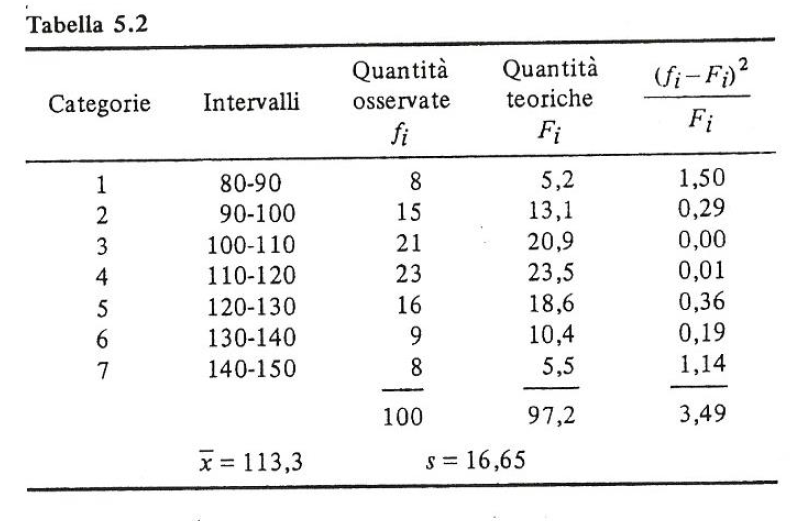
\includegraphics[width=15cm, keepaspectratio]{img/esercizio_good_fit.png}
	\caption{Tabella esempio stima distribuzione.}\label{fig:good_fit}
\end{figure}
Innanzitutto bisogna controllare il numero di osservazioni se è maggiore di $n>30$ allora possiamo applicare il metodo, inoltre suddividendo i campioni in categorie dobbiamo controllare che ci siano almeno 5 $f_i > 5$osservazioni per categoria.\\
Calcoliamo la media del campione $\bar{x}$
\[ \bar{x} = \dfrac{1}{n} \sum_{i=1}^{n} x_i = \dfrac{85\cdot8 + 95 \cdot 15 + 105 \cdot21 + 115 \cdot 23 +125 \cdot 16 + 135 \cdot9 + 145 \cdot8 }{100} = 113,3\]
Calcoliamo la deviazione standard dalla varianza $s$

\begin{equation*}
     s= \sqrt{s^2} = \sqrt{\begin{multlined}[b] 
     \dfrac{1}{n-1} \cdot [ (85\cdot8)^2 + (95 \cdot 15)^2 +\\
     (105 \cdot21)^2 +( 115 \cdot 23)^2 +(125 \cdot 16)^2 +\\
     (135 \cdot9)^2 + (145 \cdot8)^2 = 16,65]
     \end{multlined}}
\end{equation*}
    
Poi facciamo il rapporto fra le due ovvero
\[\nu = \frac{16}{113}\]
Essendo che è una normale il rapporto è un numero lontano da 1, al contrario di una esponenziale negativa.